Recurrent Neural Network (RNN) is distinguished by its memory, which can handle input sequences of any length. Its past predictions influence influence the current output. Resulting in different predictions depending on previous inputs in the sequence \cite{rnnDSmedium}.

RNNs are widely used in fields like speech recognition, image captioning, natural language processing, and language translation and are found in popular applications such as Siri, Google Translate, and Google Voice search \cite{ibmrnn}.

To illustrate how RNNs use previous inputs, consider the idiom "feeling under the weather." To understand the meaning, the words must be in a specific order. RNNs take into account the order of the words and use the information from each word to predict the next word in the sequence. Each time step represents a single word, so for example, the third time step represents "the." The hidden state of the RNN holds information from previous inputs, such as "feeling" and "under" \cite{ibmrnn}.

\begin{figure}[h]
    \centering
    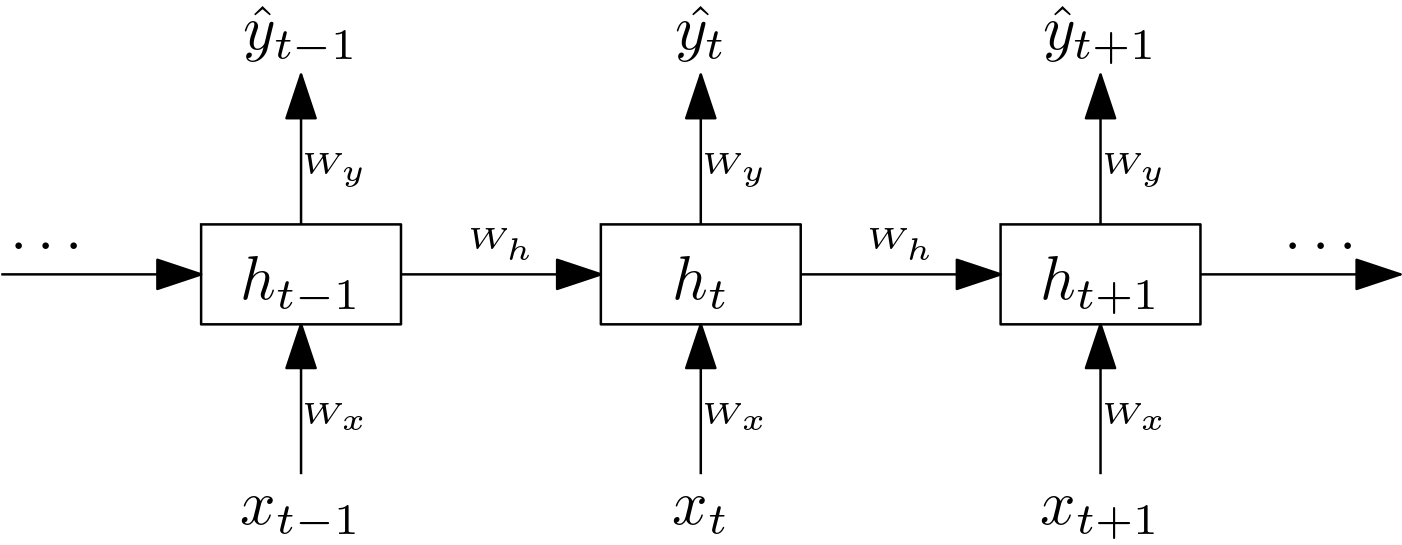
\includegraphics[width=12cm]{rnn_u.png}
    \caption{Unrolled structure of RNN \cite{matous}}
    \label{fig:rnn}
\end{figure}


Figure \ref{fig:rnn} depicts how the RNN network operates at each time step $t$. The current input $\vec{x_t}$ is processed by the network to produce the output $\hat{y}_t$, the next timestep of the input is $x_{t+1}$ with additional input from the previous time step from the hidden state $h_{t}$. This allows the neural network to have a context from previous inputs while processing the current input. The ability to hold past values and work with a context in the data is due to the recurrent units, reffered to as memory \cite{rnnin6}.

The recurrent unit is calculated as follows:

\begin{equation}
    {h_t = f(W_{x}x_t + W_{h}h_{t-1}+\vec{b_h})}
\end{equation}

$f$ is the activation function, $W_x,W_h$ are weight matrixes, $x_t$ is the input, and $\vec{b_h}$ is the vector of bias parameters. The hiddent stat $h_t$ at time step $t=0$ is initialized to $(0,0,...,0)$. The output $\hat{y_t}$ is then calculated as:

\begin{equation}
    {\hat{y}_t = g(W_{y}h_t + \vec{b_y})}
\end{equation}

$g$ is also an activation function, typically softmax, ensuring the output is in the desired class range. $W_y$ is the weight matrix, and $\vec{b_y}$ is a vector of biases determined during the learning process.

Training RNNs uses a modified version of the backpropagation algorithm called \textit{backpropagation through time} (BPTT). This process works by unrolling the RNN \cite{Goodfellow-et-al-2016}, computing the losses across each time step, and then using the backpropagation algorithm to update the weights. More on RNN in \cite{lipton2015critical} by Lipton et al.

